\documentclass{article}
\usepackage[utf8]{inputenc}
\usepackage{graphicx}
\usepackage{hyperref}
\usepackage{multirow}
\usepackage{amsmath}

\title{Research Methodology UE18CS400SG \\ Unit 3}
\author{Aditeya Baral}
\date{March 2022}

\begin{document}

\maketitle

\section{Hypothesis Testing}

\textit{"Proposition or a set of proposition set forth as an explanation for the
occurrence of some specified group of phenomena either asserted merely
as a provisional conjecture to guide some investigation or accepted as
highly probable in the light of established facts."}

\begin{itemize}
    \item An assumption or supposition to prove or disprove
    \item Suggests experiments and observations
    \item Principle Instrument of Research
    \item Used to decide if sample data can offer support for hypothesis to be generalized
\end{itemize}

\subsection{Characteristics of Hypothesis}

\begin{itemize}
    \item Clear and precise, stated in simple terms, easily understandable
    \item States relationship between variables
    \item Limited in scope and specific
    \item Consistent with facts
    \item Possible to test within reasonable time
    \item Capable of being tested (a hypothesis is testable if other deductions can be made from it which in turn can be proved or disproved)
\end{itemize}

\subsection{Basic Concepts}

\subsubsection{Null and Alternate Hypothesis}

\textbf{Null Hypothesis ($H_0$)} compares two methods and both are equally good. \textbf{Alternate Hypothesis ($H_1$)} proves one method is better than the other.

\subsubsection{Statistically Significant}

\begin{itemize}
    \item Test whether relationship between two categorical variables in a sample is also present between the two variables in the population
    \item \textbf{If the relationship is strong in the sample, it indicates the relationship in the population is real and as strong as (or even more then) the sample} -- cannot be due to \textit{chance}
    \item \textbf{Level of Significance ($\alpha$)} -- Probability of rejecting Null Hypothesis when it is actually true (conclude a difference exists when there is no difference)
\end{itemize}

\subsubsection{Type 1 and Type 2 Errors}

\begin{enumerate}
    \item \textbf{Type 1}
    \begin{itemize}
        \item \textbf{Null Hypothesis is rejected when it is true} (reject hypothesis when it should have been accepted)
        \item Results in \textbf{False Positives}
        \item $\alpha$; related to $p$ value
        \item Probability distributed at tails of a normal curve
    \end{itemize}
    \item \textbf{Type 2}
    \begin{itemize}
        \item \textbf{Null Hypothesis is accepted when it is untrue} (accept hypothesis when it should have been rejected)
        \item Results in \textbf{False Negative}
        \item $\beta$; related to \textit{power}
        \item Occurs when sample size is too small
    \end{itemize}
\end{enumerate}

\begin{table}[]
\centering
\resizebox{\textwidth}{!}{%
\begin{tabular}{lc|ll|}
\cline{3-4}
\multicolumn{2}{l|}{\multirow{2}{*}{}}                       & \multicolumn{2}{c|}{Actual}                                                                                                                                                 \\ \cline{3-4} 
\multicolumn{2}{l|}{}                                        & \multicolumn{1}{c|}{$H_0$ True}                                                                    & \multicolumn{1}{c|}{$H_0$ False}                                             \\ \hline
\multicolumn{1}{|c|}{\multirow{2}{*}{Predicted}} & Accept $H_0$ & \multicolumn{1}{l|}{\begin{tabular}[c]{@{}l@{}}No Error\\ Probability = 1 - $\alpha$\end{tabular}} & \begin{tabular}[c]{@{}l@{}}Type 2 Error\\ Probability = $\beta$\end{tabular} \\ \cline{2-4} 
\multicolumn{1}{|c|}{}                           & Reject $H_0$ & \multicolumn{1}{l|}{\begin{tabular}[c]{@{}l@{}}Type 1 Error\\ Probability = $\alpha$\end{tabular}} & \begin{tabular}[c]{@{}l@{}}No Error\\ Probability = 1 - $\beta$\end{tabular} \\ \hline
\end{tabular}%
}
\caption{Distribution of Type 1 and Type 2 Errors}
\end{table}

\subsection{One-Tailed and Two-Tailed Tests}

\begin{itemize}
    \item $\ne$ in $H_1$ -- Two-Tailed
    \item $>$ in $H_1$ -- Right-Tailed
    \item $<$ in $H_1$ -- Left-Tailed
    \item If significance is $\alpha$
    \begin{itemize}
        \item Obtain $Z$ test statistic
        \begin{equation}
            Z = \frac{\overline{X} - \mu}{\frac{\sigma_p}{\sqrt{n}}}
        \end{equation}
        \item Obtain probability $P$ from $Z$-table
        \item Reject $H_0$ (Statistically Significant) if
            \begin{itemize}
                \item For One-Tail Tests, $P < \alpha$
                \item For Two-Tail Tests, $P < \alpha/2$
            \end{itemize}
    \end{itemize}
\end{itemize}

\begin{figure*}[htp]
    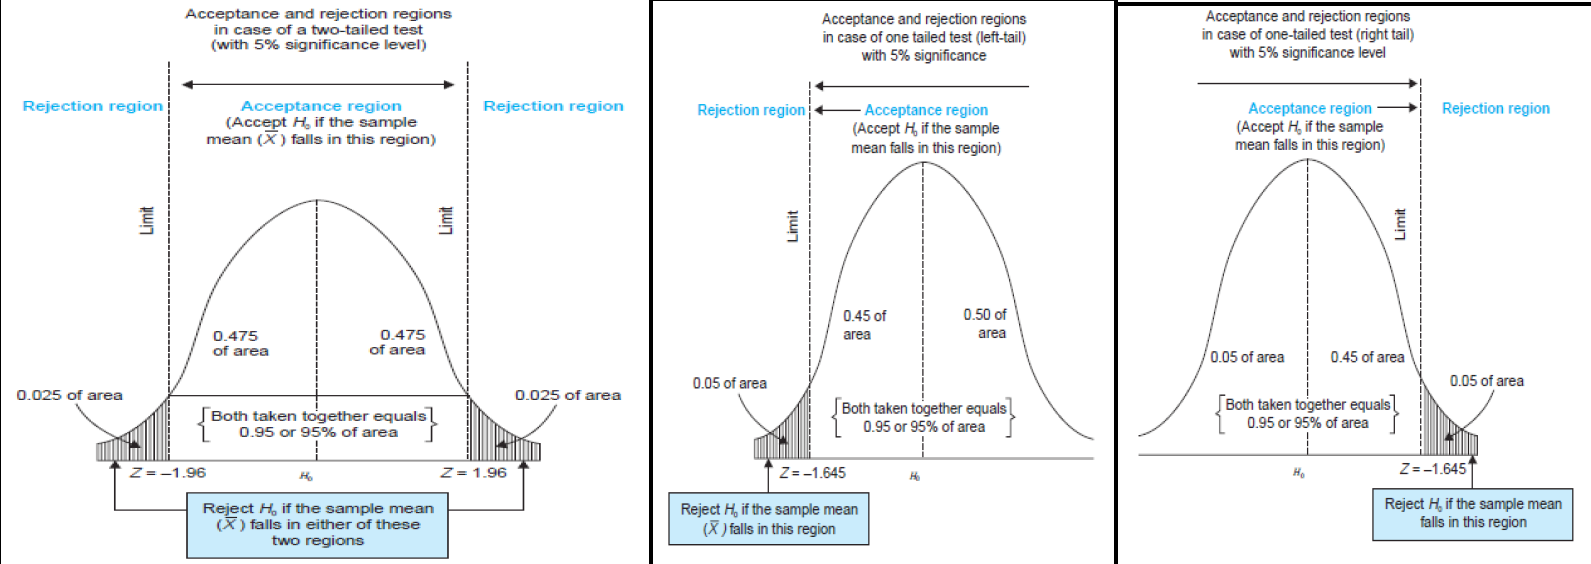
\includegraphics[width=1 \linewidth]{img/tail-tests.png}
    \caption{One-Tail and Two-Tail Acceptance and Rejection Regions}
    \label{fig:tail-test}
\end{figure*}

\subsection{Steps in Hypothesis Testing}

\begin{itemize}
    \item State $H_0$ and $H_1$
    \item Specify $\alpha$
    \item Decide sampling distribution
    \item Sample and obtain value from sample data
    \item Obtain probability that sample result will diverge from expectation if $H_0$ is true
    \item Accept or reject $H_0$ based on $P$ and $\alpha$
\end{itemize}

\subsection{Power of Hypothesis Test}

\begin{itemize}
    \item $Power = 1 - \beta$
    \item \textbf{Power is the probability of rejecting the Null Hypothesis (or accepting Alternate Hypothesis) when the Alternate Hypothesis is true}
    \item The ability to test the existence of an effect
    \item High power is desired ($\ge$80\%) -- if power value is less, increase sample size
\end{itemize}

\subsection{Types of Tests}

\subsubsection{Z-test}

Normal, infinite population, \textbf{small or large sample size}, \textbf{known variance}, $H_1$ one or two-sided

\subsubsection{t-test}

Normal, infinite population, \textbf{small sample size only}, \textbf{unknown variance}, $H_1$ one or two-sided

\begin{equation}
            t = \frac{\overline{X} - \mu}{\frac{\sigma_s}{\sqrt{n}}}
\end{equation}

\subsubsection{Chi-Square test}

\begin{itemize}
    \item Determines if sample data matches population
    \item Obtain confidence interval estimate of \textit{unknown population variance}
    \item \textbf{Non-parametric test} and \textbf{no assumptions about population}
    \item Used to test --
    \begin{itemize}
        \item \textbf{Goodness of Fit} -- how well does a theoretical distribution (binomial, poisson, normal, etc) fit the data
        \item \textbf{Independence} -- explain if two variables are dependent or associated
    \end{itemize}
    \item \textbf{Conditions for chi-square test} --
    \begin{itemize}
        \item Observations are random and independent
        \item Each group's frequency is $\ge 10$. Join groups if frequency is $< 10$
        \item Overall number of observations is large ($> 50$)
        \item Linear constrains
    \end{itemize}
    \item \textbf{Degrees of Freedom} -- Number of independent values which are assigned to a statistical distribution. 
    \begin{itemize}
        \item If we have a set of $n$ possible values, $df = n -1 $
        \item If we have an $r \times c$ matrix of values, $df = (r-1)(c-1)$
    \end{itemize}
    \item \textbf{Steps in chi-square test} (refer \href{https://www.simplilearn.com/tutorials/statistics-tutorial/chi-square-test}{this link} for solved example)
    \begin{itemize}
        \item $H_0$ states that the two variables are related. $H_1$ states that the two variables are unrelated
        \item Find Expected table $E$ using Observed table $O$
        \begin{equation}
            E_{ij} = \frac{row_i\ total \times column_j\ total}{Total\ observations}
        \end{equation}
        Or for a single event, 
        \begin{equation}
            E_{i} = P(i) \times {Total\ observations}
        \end{equation}
        \item Find $\chi^2_{calculated}$
        \begin{equation}
            \chi^2_{calculated} = \sum \frac{(O_{ij} - E_{ij})^2}{E_{ij}}
        \end{equation}
        \item For the given degrees of freedom $df$ and level of significance $\alpha$, find value of $\chi^2$ from the $\chi^2$ table
        \item If $\chi^2_{calculated} > \chi^2$, reject $H_0$
    \end{itemize}
\end{itemize}

\section{ANOVA -- ANalysis Of VAriance}

\subsection{Hypothesis Testing with $> 1$ Samples or Populations}

\begin{itemize}
    \item It is used to find the \textbf{variability between sample means}
    \item Helps determine if \textit{samples are from the same larger population}
    \item Multiple t-tests or z-tests are not the answer
    \begin{itemize}
        \item \textit{Increased} number of tests $\binom{n}{2}$
        \item Error \textit{compounds} with each test -- if confidence level is 95\% and $n$ tests are conducted, the confidence is $0.95^n$ (large decrease), and hence $\alpha = 1 - 0.95^n$ (large increase)
    \end{itemize} 
\end{itemize}

\subsubsection{Equations for Z and t statistic for 2 Samples or Populations}

\begin{equation}
    z = \frac{\overline{X_1} - \overline{X_2}}{\sqrt{\frac{\sigma_1^2}{n_1} + \frac{\sigma_2^2}{n_2}}}
\end{equation}

\begin{equation}
    t = \frac{\overline{X_1} - \overline{X_2}}{\sqrt{\frac{\sum_{i=1}^{n_1} (X_{1i} - \overline{X_1}) + \sum_{i=1}^{n_2} (X_{2i} - \overline{X_2})}{n_1 + n_2 - 2}} \times \sqrt{\frac{1}{n_1} + \frac{1}{n_2}}}
\end{equation}

\subsection{Obtaining ANOVA Table}

\textbf{Overall Mean ($\overline{\overline{X}}$)} is the mean of all possible data points ($x_{i}^{(j)}$) across populations or samples. If $N = n_1 + n_2 + n_3 + ... + n_P$, then

\begin{equation}
    \overline{\overline{X}} = \frac{\sum_{i=1}^{N} x_i}{N},\ or\ \overline{\overline{X}} = \frac{\sum_{i=1}^{P}\sum_{j=1}^{n_i} x_{i}^{(j)}}{\sum_{i=1}^{P}n_i}
\end{equation}

\textbf{Total/Overall Sum of Squares (SST)} or \textbf{SS for Total Variance} is the summation of the squares of the differences between every data point ($x_{i}^{(j)}$) and the overall mean ($\overline{\overline{X}}$). It is also the \textbf{sum of the variance within and variance between}.

\begin{equation}
    SST = \sum_{i=1}^{P}\sum_{j=1}^{n_i} (x_{i}^{(j)} - \overline{\overline{X}})^2
\end{equation}

\begin{equation}
    SST = SSC + SSE
\end{equation}

\textbf{Column/Between Sum of Squares (SSC)} is the summation of the squares of the differences between the population or sample mean ($\overline{X_i}$) and overall mean ($\overline{\overline{X}}$)

\begin{equation}
    SS\ Between = \sum_{i=1}^{P} n_i (\overline{X_i} - \overline{\overline{X}})^2
\end{equation}

\textbf{Mean Squares Between (MS Between)} is the ratio between SSC and its degree of freedom

\begin{equation}
    MS\ Between = \frac{SSC}{P - 1}
\end{equation}

\textbf{Error/Within Sum of Squares (SSE)} is summation of the squares of the differences between every data point ($x_{i}^{(j)}$) and its population or sample mean ($\overline{X_i}$)

\begin{equation}
    SSE = \sum_{i=1}^{P}\sum_{j=1}^{n_i} (x_{i}^{(j)} - \overline{X_i})^2
\end{equation}

\textbf{Mean Squares Within (MS Within)} is the ratio between SSE and its degree of freedom

\begin{equation}
    MS\ Within = \frac{SSE}{\sum_{i=1}^{P}n_i - P}
\end{equation}

\textbf{\textit{F}-ratio} is the ratio between MS Between and MS Within

\begin{equation}
    F-ratio = \frac{MS\ Between}{MS\ Within}
\end{equation}

\begin{table}[h]
\centering
\begin{tabular}{|l|l|l|ll}
\hline
\textbf{Variation} & \textbf{SS} & \textbf{df} & \multicolumn{1}{l|}{\textbf{MS}} & \multicolumn{1}{l|}{\textbf{F-ratio}}                       \\ \hline
Between            & SSC         & P - 1       & \multicolumn{1}{l|}{$\frac{SSC}{P - 1}$} & \multicolumn{1}{l|}{\multirow{2}{*}{$\frac{MS\ Between}{MS\ Within}$}} \\ \cline{1-4}
Within             & SSE         & N - P       & \multicolumn{1}{l|}{$\frac{SSE}{N - P}$}  & \multicolumn{1}{l|}{}                                       \\ \hline
Total              & SST         & N - 1       &                                  &                                                             \\ \cline{1-3}
\end{tabular}
\caption{ANOVA Table}
\label{tab:anova}
\end{table}

\textbf{\textit{P}-value} can be obtained from the F-table. If \textit{P}-value is less than $\alpha$, then we reject $H_0$.

\begin{equation}
    P-value = P(df_{between}, df_{within})
\end{equation}

\section{Data Representation}

Organization of data into tables, graphs or charts, so that logical and statistical conclusions can be derived from the collected measurements. Can be in the form of text, tables or graphs, help present and convey information
\begin{itemize}
    \item Table -- data organized orderly in rows and columns
    \item Visual/Figure -- presentation like charts, graphs, diagrams, maps etc
\end{itemize}

\subsection{Tabular Presentation}

\begin{itemize}
    \item Data presented orderly in rows and columns, based on characteristics
    \item 2D, each row/record represents an entity, each column is attribute and is unique
    \item Compact and self-explanatory, easier to comprehend and understand
    \item Numeric tables - store quantitative, or combination of quantitative and qualitative data (mostly numeric values)
    \item Table Types
    \begin{itemize}
        \item \textbf{Purpose} -- reference table, text table
        \item \textbf{Content}
        \begin{itemize}
            \item Simple -- one characteristic per stub
            \item Complex -- double (2 characteristics per stub), triple (3 characteristics), multiple (each stub may be further divided into characteristics)
        \end{itemize}
    \end{itemize}
    \item Components -- table number (to identify and reference tables), title, stub (row heading), caption (column heading), body, foot note, source note
\end{itemize}

\begin{figure*}[htp]
    \centering
    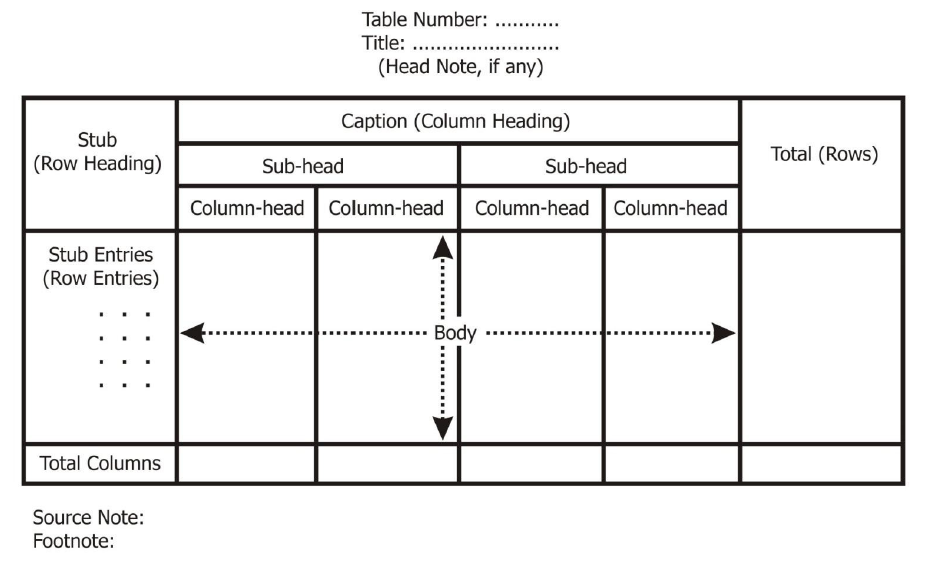
\includegraphics[width=0.8 \linewidth]{img/table.png}
    \caption{Components of a Table}
    \label{fig:tail-test}
\end{figure*}

\subsubsection{Advantages of Table}

\begin{itemize}
    \item Represents large amount of data in an orderly manner
    \item Easy to read, organized in rows and columns
    \item Easy to construct
    \item Easy to add new records (as rows)
\end{itemize}

\subsubsection{Features of a Good Table}
\begin{itemize}
    \item Attractive
    \item Simple, clear, easy to understand
    \item Avoid too many details, should not be too big or too small
\end{itemize}

\subsection{Graphs and Diagrams}

Used to represent data in visual form, supported by narration from presenter. Graphs can be either histogram, frequency curve ogive (cumulative frequency) or line graphs. Diagrams include bar plot and pie chart.

\begin{table}[h]
\centering
\begin{tabular}{|l|l|}
\hline
\textbf{Graphs}                                                                                    & \textbf{Diagrams}                                                                                          \\ \hline
Graph paper used                                                                                   & Plain paper used                                                                                           \\ \hline
\begin{tabular}[c]{@{}l@{}}Shows mathematical relationship\\ between two variables\end{tabular}    & Does not show any relationship                                                                             \\ \hline
\begin{tabular}[c]{@{}l@{}}Appropriate for frequency distributions \\ and time series\end{tabular} & Not suitable for such data                                                                                 \\ \hline
Not attractive                                                                                     & \begin{tabular}[c]{@{}l@{}}More attractive and suitable for \\ publicity and propaganda\end{tabular}       \\ \hline
Adds meaning to data and aids analysis                                                             & \begin{tabular}[c]{@{}l@{}}Do not add to the meaning of data and \\ does not help in analysis\end{tabular} \\ \hline
\begin{tabular}[c]{@{}l@{}}Used by statisticians and \\ research workers in analysis\end{tabular}  & Used to display data in different ways                                                                     \\ \hline
\end{tabular}
\caption{Difference between Graphs and Diagrams}
\label{tab:graph-diagram}
\end{table}

\subsubsection{Rules for Drawing Graphs and Diagrams}

\begin{itemize}
    \item Choose appropriate form of visualization
    \item Title -- information about graph
    \item Scale and units -- neither too big or small, use right units
    \item Neat, attractive, simple to interpret and convey meaning
    \item Original
    \item Economical -- should not be laborious or costly to construct
\end{itemize}

\subsubsection{Advantages of Graphs and Diagrams}

\begin{itemize}
    \item Attractive and long-lasting impression
    \item Bird's eye view of data
    \item Easy to understand and compare characteristics
    \item Graphs help visualize theorems and results of statistics
\end{itemize}

\subsubsection{Limitations of Graphs and Diagrams}

\begin{itemize}
    \item Visual aids cannot replace numerical data
    \item Lack of mathematical rigour
    \item Not as accurate as tabular data
    \item Misrepresentation in visualization leads to misled observers and wrong interpretations
\end{itemize}

\section{Results and Discussion -- Data Interpretation}

\subsection{Results}

\textbf{Results} are what you find in research, \textit{without details, interpretation or references to literature}. Focuses on facts and presents a simple and clear account of what was achieved

\subsection{Discussion}

\textbf{Discussion} is the heart of the paper and commentary of results. It addresses the meaning of the findings in research.

\begin{itemize}
    \item \textbf{Purpose} -- state interpretations, opinions, implications of findings and suggestions for future research
    \item \textbf{Function} -- answer questions in introduction, explain how results support answers and how answers fit with existing knowledge. If results are not in the desired direction, explain why (sampling, measurement, procedure, confounding variables etc)
    \begin{itemize}
        \item Summarize previous findings and then your findings
        \item Provide meaningful answers
        \item Interpret objectively and subjectively
        \item Include references to others' interpretations
        \item Every conclusion should be defensible
    \end{itemize}
    \item \textbf{Include} -- unexpected results, references to previous research, explanations, exemplifications, deductions, hypothesis and recommendations
\end{itemize}

\subsubsection{Technique of Discussion}

\begin{enumerate}
    \item \textbf{Organize Discussion} -- specific to general, $findings \rightarrow literature \rightarrow theory \rightarrow practice$
    \item \textbf{Re-state Hypothesis} and answer questions in introduction
    \item \textbf{Explain results} -- are they expected, why are they acceptable, how are they consistent with published knowledge
    \item \textbf{Address all results} -- regardless of statistical significance
    \item \textbf{Describe patterns, principles and relationships} -- State answer, then support with results, then cite other work
    \item \textbf{Defend answers} -- why is the work satisfactory, why is others' work not suitable, give convincing reasons
    \item \textbf{Discuss and evaluate conflicting explanations}
    \item \textbf{Discuss unexpected findings} -- mention finding and then describe
    \item \textbf{Identify limitations and weaknesses} -- are they important to interpretation of results, do they affect validity of findings, no apologetic tone
    \item \textbf{Summarize} -- concise, brief, specific, importance and implication, recommendations for future research
\end{enumerate}

\begin{table}[h]
\centering
\begin{tabular}{|l|l|}
\hline
\textbf{Do's}                   & \textbf{Don't's}     \\ \hline
Provide context and explanation & Rehash results       \\ \hline
Emphasize positives             & Exaggerate positives \\ \hline
Look towards the future         & End with it          \\ \hline
\end{tabular}
\caption{Do's and Don't's of writing a Discussion}
\label{tab:dos-donts-discussion}
\end{table}

\section{Summary, Conclusion and Recommendation}

\subsection{Summary}

\textbf{Summary} is a restatement of findings under each factor.

\begin{itemize}
    \item Summarizes findings
    \item May be the conclusion too
    \item Limitations and future work
\end{itemize}

\subsection{Conclusion}

\textbf{Conclusion} is an \textit{interpretation (not repetition)} of facts discussed. It is a take-away from the study, bounded by what is shown in data. Highlights the value and point of the study.

\subsubsection{Purpose of Conclusion}

\begin{itemize}
    \item Integrate issues raised in discussion
    \item Reflect on introduction, problem statement and objectives
    \item Answer research questions
    \item Identify theoretical implications of study
    \item Highlight limitations
    \item Direction for future research
\end{itemize}

\subsubsection{Content of a Good Conclusion}

\begin{itemize}
    \item Logical ending, integrates what was discussed
    \item No new or undiscussed information
    \item Pulls together all parts of the argument
    \item Refers the reader to the focus or central topic of the study
    \item Systematic and brief
    \item Adds to overall quality and impact of study
    \item Consists of the following
    \begin{itemize}
        \item Restate research questions -- reinforce importance
        \item Empirical findings
        \item Theoretical implications
        \item Recommendations for future research
        \item Limitations
    \end{itemize}
\end{itemize}

\section{References}

A \textbf{referencing style} is a specific format for presenting in-text references (footnotes or endnotes) and bibliography. A \textbf{reference} is the action of mentioning or alluding a source of information to ascertain something.

The \textbf{types of references} are \textbf{journal, book and internet}. \textbf{Reference elements} include \textbf{Authors' names, title, journal name, year, volume and page numbers}

\subsection{Reasons for Referencing}

\begin{itemize}
    \item Proves research has been done to support analysis
    \item Easy to follow up on work
    \item Credit to others' work
    \item Avoids plagiarism charges
    \item Needed to support all significant statements
    \item Indicates origin of material and source of research (for further reading)
\end{itemize}

\subsection{Styles of Referencing}

\footnote{Not needed for ISA. Memorize before ESA}

\subsubsection{Harvard Style}

\begin{enumerate}
    \item Author’s name followed by its initials
    \item Year of publication
    \item Article title with single quotation mark followed by full stop
    \item Name of Journal in italic form
    \item Volume followed by a comma
    \item Issue no. in bracket
    \item Page no
\end{enumerate}

\subsubsection{Vancouver Style}

\begin{enumerate}
    \item Author Surname followed by Initials
    \item Title of article followed by double quotation
    \item Title of journal (abbreviated)
    \item Date of Publication followed by semicolon
    \item Volume Number
    \item Issue Number in bracket
    \item Page Number
\end{enumerate}

\subsubsection{MLA Citation Style (Modern language Association)}

\begin{enumerate}
    \item Authors name
    \item Title of article
    \item Name of journal
    \item Volume number followed by decimal & issue no
    \item Year of publication
    \item Page numbers
    \item Medium of publication
\end{enumerate}

\subsubsection{American Psychological Association Style (APA)}

\begin{enumerate}
    \item Author’s name followed by its initials
    \item Year of publication
    \item Article title followed by full stop
    \item Name of Journal in italic form
    \item Volume followed by a comma
    \item Page no
\end{enumerate}

\subsubsection{Chicago Manual Style}

\begin{enumerate}
    \item Name of author
    \item Article title in double quotation mark
    \item Title of journal in italic
    \item Volume
    \item Year of publication
    \item Page no
\end{enumerate}

\subsubsection{Royal Society of Chemistry}

\begin{enumerate}
    \item Initials followed by author’s surname
    \item Title of journal (abbreviated)
    \item Year of publication
    \item Volume number
    \item Pages no
\end{enumerate}

\subsection{Difference between Reference List and Bibliography}

\begin{table}[h]
\centering
\begin{tabular}{|l|l|}
\hline
\textbf{Reference List}                                                                                & \textbf{Bibliography}                                                                        \\ \hline
Sources cited in text                                                                                  & \begin{tabular}[c]{@{}l@{}}Sources consulted for study but may\\ not be cited\end{tabular}   \\ \hline
Arranged in citation order                                                                             & \begin{tabular}[c]{@{}l@{}}Arranged in alphabetical order of \\ author surnames\end{tabular} \\ \hline
\begin{tabular}[c]{@{}l@{}}Placed at the end of the paper, \\ or as a footnote or endnote\end{tabular} & Placed at the end of the paper                                                               \\ \hline
\end{tabular}
\caption{Difference between Reference List and Bibliography}
\label{tab:reflist-vs-bib}
\end{table}

\end{document}
